\begin{flushright} {\tiny {\color{gray} geo1427project.tex}} \end{flushright}
%~~~~~~~~~~~~~~~~~~~~~~~~~~~~~~~~~~~~~~~~~~~~~~~~~~~~~~~~~~~~~~~~~~~~~~~~~~~~


We consider a 2D Cartesian domain. We wish to solve the incompressible 
isothermal Stokes equations in this domain using the 
vorticity-streamfunction approach (see Section~\ref{ss:vorticitystreamfunction}). 
We assume that the fluids in the domain all have the same viscosity 
$\eta_0$ and that the gravity is vertical 
and pointing downwards, i.e.  $\vec{g}=(g_x,g_y)=(0,-g_0)$.
The density in the domain is given by a  function $\rho(x,y)$ specified
here after. In what follows the boundary conditions are assumed to be free slip. 

\begin{itemize}
\item
Experiment 1: the domain is a square of size 600~\si{\km}.  
It contains two fluids, the `mantle'  and the `slab'. 
The mantle has a density of 3200~\si{\kg\per\cubic\meter} 
and fills the domain except for a circle (the slab) of radius 100~\si{\km} 
centered at $x=L_x/2$ and $y=\frac23 L_y$  of density 
3300~\si{\kg\per\cubic\meter}. $g_0=10~\si{\meter\per\square\second}$ 
and $\eta_0=10^{21}~\si{\pascal\second}$.

\begin{center}
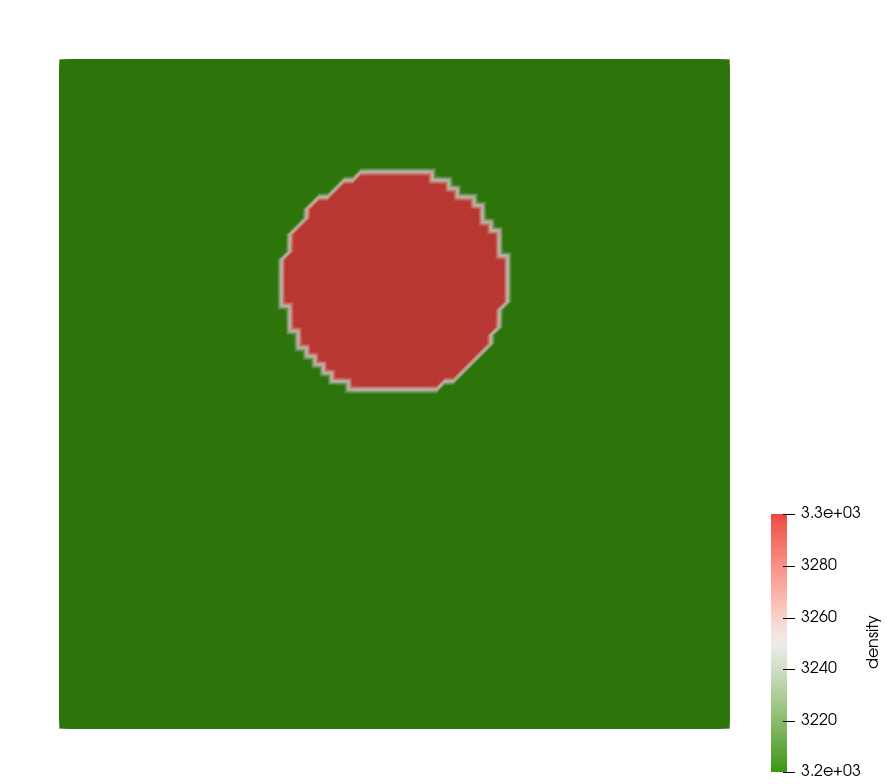
\includegraphics[width=5cm]{images/fdm/project/rho1}
\end{center}

\item
Experiment 2: 
gravity field ($g_x=0$, $g_y=10~\si{\meter\per\square\second}$) 
for a density structure with two vertical layers 
(3200~\si{\kg\per\cubic\meter} and 3300~\si{\kg\per\cubic\meter} 
for the left and right layers, respectively). The model size is  
$1500~\si{\km} \times 1000~\si{\km}$.
Use a constant viscosity $\eta = 10^{21}~\si{\pascal\second}$ 
for the entire model.
\end{itemize}

\begin{center}
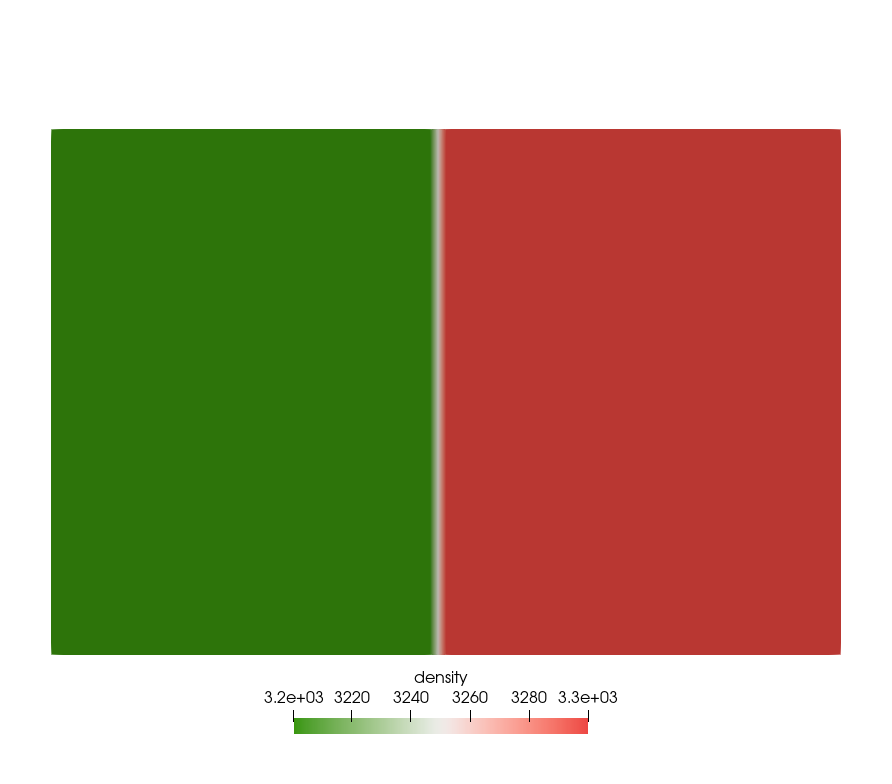
\includegraphics[width=5cm]{images/fdm/project/rho2}
\end{center}

%--------------------------------
\subsection*{Background theory}

We start from 
\begin{equation}
\vec\nabla^4 \psi = \frac{1}{\eta_0} \left( -\frac{\partial (\rho g_x)}{\partial y}
+\frac{\partial (\rho g_y)}{\partial x} \right)
\label{eq:md40XX}
\end{equation}
where
\[
\vec\nabla^4 = 
\left( 
\frac{\partial^2 }{\partial x^2} + \frac{\partial^2 }{\partial y^2} 
\right) 
\left( 
\frac{\partial^2 }{\partial x^2} + \frac{\partial^2 }{\partial y^2} 
\right) 
\]
Eq.~\eqref{eq:md40XX} can be rewritten as two Poisson equations, by 
defining the vorticity as $\omega = \vec\nabla^2 \psi$:

We obtain 
the Poisson equation for the vorticity $\omega$:
\begin{equation}
\vec\nabla^2 \omega = -\frac{1}{\eta_0} \left( -\frac{\partial (\rho g_x)}{\partial y}
+\frac{\partial (\rho g_y)}{\partial x} \right)
\end{equation}
In what follows we assume that the domain is a Cartesian box aligned 
with the $x,y$ axis. The gravity is constant and vertical so that $g_x=0$ and 
then we must solve 
\begin{eqnarray}
\vec\nabla^2 \omega &=& -\frac{g_0}{\eta_0}  \frac{\partial \rho}{\partial x} \label{eq:poiss1} \\
\vec\nabla^2 \psi &=& \omega  \label{eq:poiss2} 
\end{eqnarray}


\begin{enumerate}
\item The domain under consideration is a rectangle of size $L_x \times L_y$. Create a mesh of $nnx \times nny$ nodes. 
Store the $x$ and $y$ coordinates in 2 arrays {\tt xcoords} and {\tt ycoords}
\item Prescribe the density $\rho$ on the nodes of the mesh, store the values in the {\tt rho} array. 
Visualise this field and produce a figure called {\sl rho.png}.
\item Compute $\partial \rho/ \partial x$ on the nodes. Visualise this field and produce a figure called {\sl drhodx.png}. 
Use a centered approach if a node is inside the domain and a backward or forward approach if it is on a boundary.
\item Solve Eq.~\eqref{eq:poiss1} using the FD method. Solve the linear system with a scipy solver. Boundary conditions for $\omega$ are $\omega=0$ on all four sides of the domain.
Visualise this field and produce a figure called {\sl omega.png}
\item Solve Eq.~\eqref{eq:poiss2} in a similar way, also setting $\psi=0$ on all four sides.
Visualise this field and produce a figure called {\sl psi.png}
\item Compute the velocity components $u$ and $v$ at each node using 
\[
u=\frac{\partial \psi}{\partial y} 
\qquad \text{and} \qquad
v=-\frac{\partial \psi}{\partial x} 
\]
As in question 2, use the appropriate stencil whether a node is on a boundary or not.
Test your implementation of the gradients by computing $u,v$ at each node having set $\psi=1$ on all nodes
(test 1) and set $\psi=xy$ on all nodes (test 2). In both cases, what values of $u,v$ do we expect? 
Do you recover these values? (if not there is a problem here and you should not proceed any further 

When this is correct, visualise the velocity components (in cm/year!) for the sinking sphere: produce then 
two files, {\sl u.png} and {\sl v.png}, and also a third file {\sl vel.png} 
with the density overlain by velocity vectors. 

\item Compute the strain rate tensor components
\[
\dot\varepsilon_{xx} =\frac{\partial u}{\partial x} 
\qquad
\dot\varepsilon_{yy} =\frac{\partial v}{\partial y} 
\qquad
\dot\varepsilon_{xy} = \frac12 \left(\frac{\partial u}{\partial y} + \frac{\partial v}{\partial x} \right)
\]
Visualise these fields and produce then three files {\sl exx.png}, {\sl eyy.png} and {\sl exy.png}.

\item Compute the effective strain rate
\[
\varepsilon_e = \sqrt{ \frac{1}{2}(\dot\varepsilon_{xx}^2 + \dot\varepsilon_{yy}^2 ) + \dot\varepsilon_{xy}^2  }
\]
and produce a figure {\sl ee.png}

\item Bonus: try the 9 point Laplace stencil, see Section~\ref{ss:ninepointstencil}.

\end{enumerate}


